\documentclass[12pt,a4paper]{article}

% ==================== PACKAGES ====================
\usepackage[utf8]{inputenc}
\usepackage[T1]{fontenc}
\usepackage{graphicx}
\usepackage{geometry}
\usepackage{setspace}
\usepackage{fancyhdr}
\usepackage{titlesec}
\usepackage{float}
\usepackage{enumitem}
\usepackage{hyperref}
\usepackage{xcolor}
\usepackage{tocloft}
\usepackage{tikz}
\usepackage{lmodern}

% ==================== PAGE SETUP ====================
\geometry{margin=1in}
\setstretch{1.25}
\setlength{\parskip}{0.5em}
\setlength{\parindent}{0pt}

% ==================== COLOR SCHEME ====================
\definecolor{primaryblue}{RGB}{25,55,109}
\definecolor{accentred}{RGB}{200,16,46}
\definecolor{lightgray}{RGB}{245,245,245}
\definecolor{textgray}{RGB}{60,60,60}

% ==================== HEADER & FOOTER ====================
\pagestyle{fancy}
\fancyhf{}
\fancyhead[L]{\small\color{primaryblue}\textit{Smart Health Monitoring System}}
\fancyhead[R]{\small\color{primaryblue}\textbf{\thepage}}
\renewcommand{\headrulewidth}{0.5pt}
\renewcommand{\headrule}{\hbox to\headwidth{\color{primaryblue}\leaders\hrule height \headrulewidth\hfill}}
\fancyfoot[C]{\small\color{gray}\textit{Higher School of Communication of Tunis}}
\renewcommand{\footrulewidth}{0pt}

% ==================== SECTION FORMATTING ====================
\titleformat{\section}
  {\LARGE\bfseries\color{primaryblue}}
  {\thesection.}{0.5em}{}
  [\vspace{0.3em}]

\titleformat{\subsection}
  {\Large\bfseries\color{primaryblue}}
  {\thesubsection}{1em}{}
  [\vspace{0.2em}]

% ==================== TABLE OF CONTENTS STYLING ====================
\renewcommand{\contentsname}{\color{primaryblue}\Huge\bfseries Table of Contents}
\renewcommand{\cftsecfont}{\large\bfseries\color{primaryblue}}
\renewcommand{\cftsubsecfont}{\normalsize\color{textgray}}
\renewcommand{\cftsecpagefont}{\large\bfseries\color{primaryblue}}
\renewcommand{\cftsubsecpagefont}{\normalsize\color{textgray}}
\renewcommand{\cftsecleader}{\cftdotfill{\cftdotsep}}
\setlength{\cftbeforesecskip}{10pt}
\setlength{\cftbeforesubsecskip}{5pt}

% ==================== HYPERLINKS ====================
\hypersetup{
    colorlinks=true,
    linkcolor=primaryblue,
    urlcolor=accentred,
    citecolor=primaryblue,
    linktoc=all
}

% ==================== TITLE PAGE ====================
\begin{document}

\begin{titlepage}
\centering
\vspace*{cm}

% Logo

\includegraphics[width=6cm]{Images/Supcom.png}

\vspace{0.5cm}

% Institution name
{\Large \textbf{Higher School of Communication of Tunis}}\\[2cm]

% Document title with decorative lines
{\color{primaryblue}\rule{0.75\textwidth}{1.2pt}}\\[0.5cm]
{\Huge \bfseries\color{primaryblue} Design Document}\\[0.5cm]
{\color{primaryblue}\rule{0.75\textwidth}{1.2pt}}\\[2.5cm]

% Project title
{\Large\color{accentred}\textbf{Smart Health Monitoring System}}\\[3cm]

% Authors
{\small \textit{Authored by:}}\\[0.4cm]
{\large Ahmed Essouaid, Aziz May, Moez Zouari, Mohamed Amine Chamtouri}\\[2cm]

% Supervisor
{\small \textit{Supervised by:}}\\[0.4cm]
{\large Dr. Eng. Mohamed-Bécha Kaaniche}\\[2cm]

% Academic year
{\small \textit{Academic Year:}}\\[0.4cm]
{\large\bfseries 2025--2026}

\vfill
\end{titlepage}

% ==================== TABLE OF CONTENTS ====================
\newpage
\pagenumbering{roman}
\setcounter{page}{1}
\thispagestyle{fancy}
\begin{center}
\vspace*{2cm}
{\Huge\bfseries\color{primaryblue} Table of Contents}\\[0.3cm]
\color{accentred}\rule{0.5\textwidth}{1.5pt}
\end{center}
\vspace{1cm}
\tableofcontents
\newpage

% ==================== MAIN CONTENT ====================
\pagenumbering{arabic}
\setcounter{page}{1}

\section{Problematic}

Healthcare systems today face several challenges. Patients with chronic illnesses or conditions requiring continuous observation often lack access to reliable monitoring outside of clinical environments. Traditional solutions are expensive, limited in scope, and unable to provide real-time feedback to healthcare professionals.

Moreover, emergencies such as falls or heart attacks are often detected too late, delaying treatment and endangering patient lives. Medical staff are also burdened with increasing patient loads, making personalized monitoring difficult to maintain.

There is therefore a pressing need for smart systems that can continuously track vital signs, apply predictive models to anticipate emergencies, and immediately notify caregivers with accurate patient data and location.

\section{Context of the Project}

This project is situated at the intersection of Internet of Things (IoT), cloud computing, and artificial intelligence. Recent advances in wearable sensors and mobile connectivity make it possible to capture vital health data outside of hospitals. At the same time, cloud services provide the scalability, storage, and computational power necessary to process and analyze this data in real time.

The integration of machine learning into health monitoring opens the door to not only detecting anomalies but also predicting critical health conditions before they become life-threatening. Within this technological context, our project demonstrates how Cloud of Things can enable smarter, more responsive healthcare solutions.

\section{Architecture}

The proposed IoT architecture presents a modern, scalable solution that seamlessly integrates edge computing capabilities with cloud infrastructure. This design emphasizes real-time data processing, robust communication protocols, and intelligent decision-making at both edge and cloud levels.

\begin{figure}[H]
    \centering
    \fcolorbox{primaryblue}{white}{%
        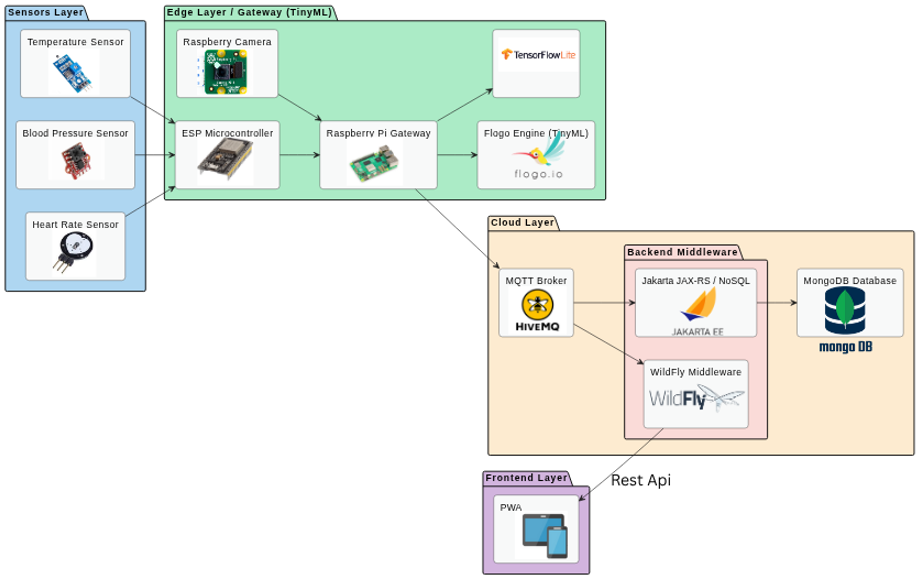
\includegraphics[width=0.92\textwidth]{Images/Iot_Architecture.png}
    }
    \caption{\textbf{IoT Architecture Overview}}
    \label{fig:architecture}
\end{figure}

\section{UML Diagrams}

\subsection{Use Case Diagram}

Figure \ref{fig:usecase} illustrates the Use Case diagram of the system, depicting the primary actors and their interactions with various system functionalities. The system accommodates four main actors: patients, healthcare professionals, family members, and system administrators, each with distinct privileges and responsibilities tailored to their role in the healthcare monitoring ecosystem.

\begin{figure}[H]
    \centering
    \fcolorbox{primaryblue}{white}{%
        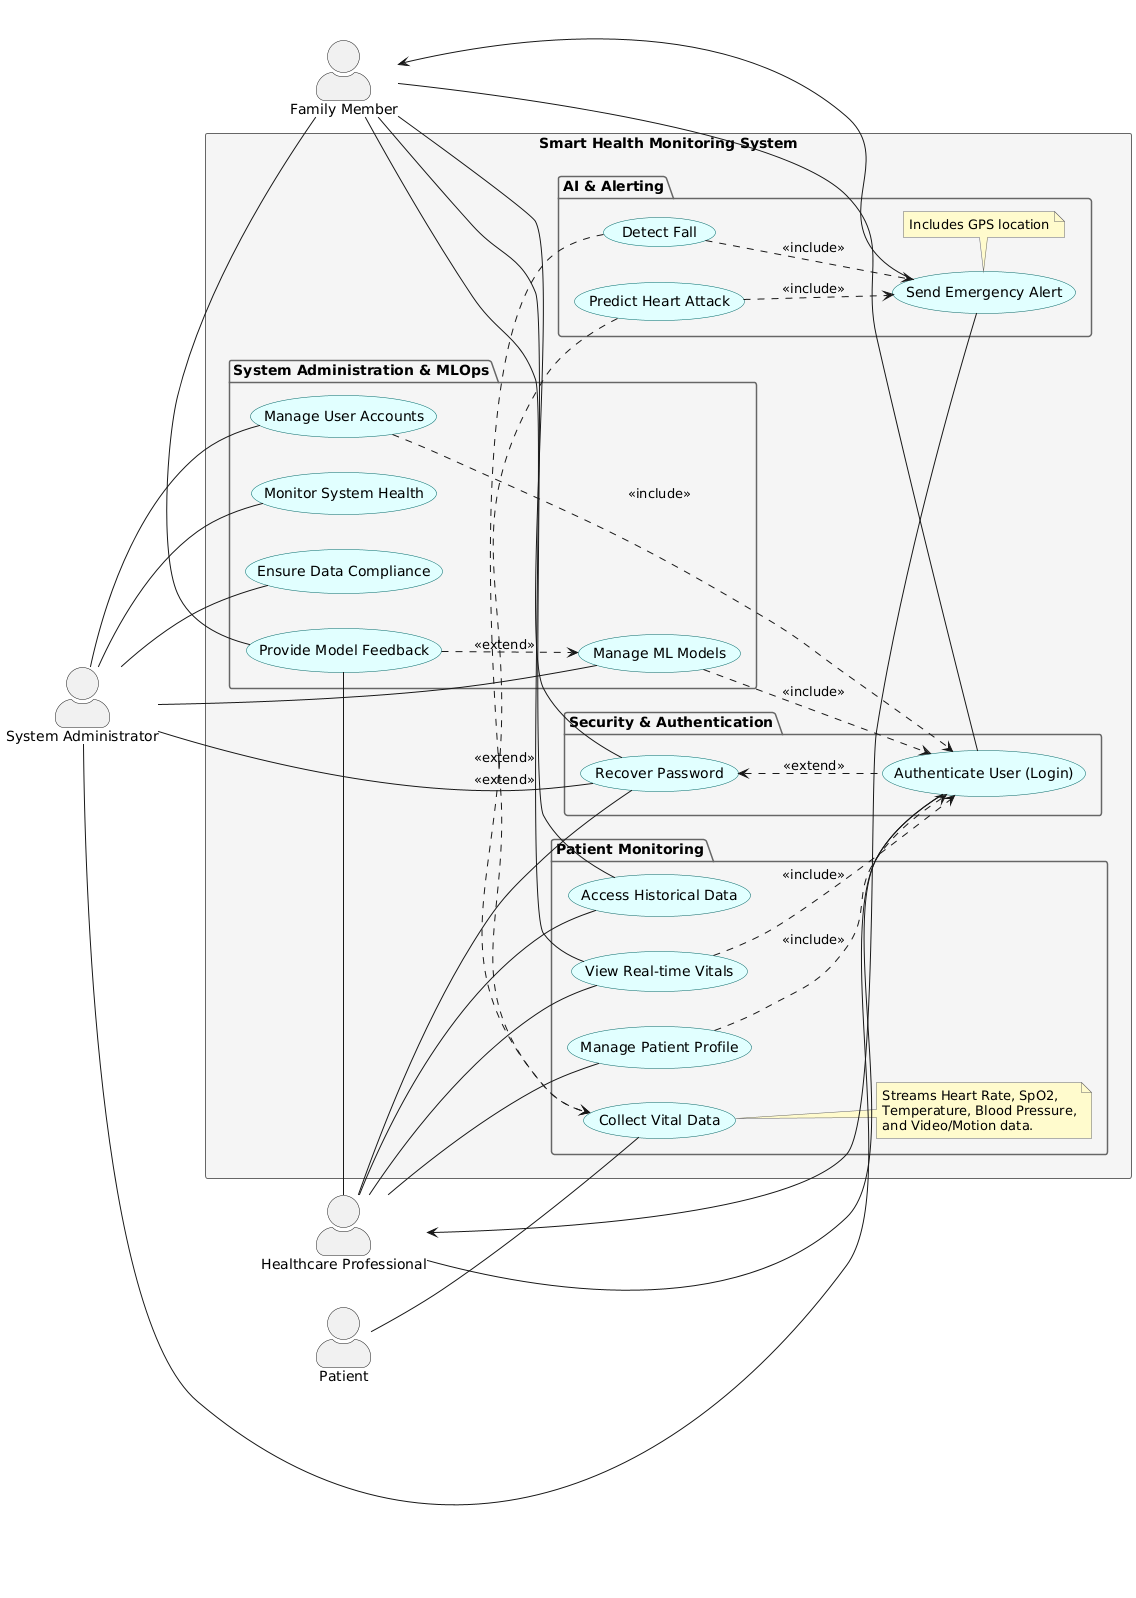
\includegraphics[width=0.92\textwidth]{Images/Use_Case.png}
    }
    \caption{\textbf{Use Case Diagram - System Actors and Interactions}}
    \label{fig:usecase}
\end{figure}

\newpage

\section*{Conclusion}
\addcontentsline{toc}{section}{Conclusion}

To be completed later

\end{document}